\section{Status of the EMC effect\label{sec:status}}
%
One of the best tools available for studying the internal structure of nucleons is the deep inelastic
scattering (DIS) process, where a charged lepton scatters inelastically with a large four-momentum
transfer, $q^\mu$, represented by the Lorentz invariant $Q^2 = -q^\mu q_\mu \gg 1-2~\mathrm{GeV}^2$.
The process is characterized by a scaling variable called Bjorken-$x$, defined by $x = Q^2/2M \nu$, 
where $M$ is the mass of the target and $\nu$ is the energy transferred from the lepton in the laboratory frame. Bjorken-$x$ is associated with the light-cone momentum fraction carried by the struck parton in the limit of the infinite-momentum frame. To leading order the unpolarized electromagnetic DIS cross-section for a spin-1/2 target such as the proton can be written as~\cite{PhysRevD.98.030001}
%
\begin{equation}
\frac{d^2 \sigma}{dx dy} = \frac{4 \pi \alpha^2}{x y Q^2} \left[ (1-y)F_2(x, Q^2) + y^2 x F_1(x, Q^2) \right],
\end{equation}
%
where $y = \nu/E$ with $E$ is the incident lepton energy, $\alpha$ is the electromagnetic fine structure constant, and $F_2$
and $F_1$ are the structure functions of the target to be determined by experiment. These structure functions can be reduced by the Callan-Gross relation $F_2 - 2xF_1 = F_\mathrm{L} \approx 0$ for non-interacting point-like spin-1/2 particles with
%
\begin{equation}
F_2(x,Q^2) = x \sum_{q} e_q^2 \left[q(x,Q^2) + \bar{q}(x,Q^2)\right],
\end{equation}
%
where the sum $q$ is over all quark flavors,  $e_q$ is the electromagnetic charge of the quark, and the functions $q(x,Q^2)$ and $\bar{q}(x,Q^2)$ are the parton distribution functions (PDFs) which are universal and can describe other processes such as Drell-Yan scattering.  The ratio of $F_L$ to $F_T$, the transverse structure function, $F_T$,  $R = F_L/F_T$ is of important interest for small $x$ and small $Q^2$ where the contributions can be sizeable from photon-gluon fusion and higher-twist corrections respectively.  This has not been as well studied for nuclear targets and often represents an open systematic uncertainty.  Analogous distributions exist for the case of polarized targets. These PDFs can in principle be measured for any bound hadronic state.

\begin{figure}[tbp]
\centering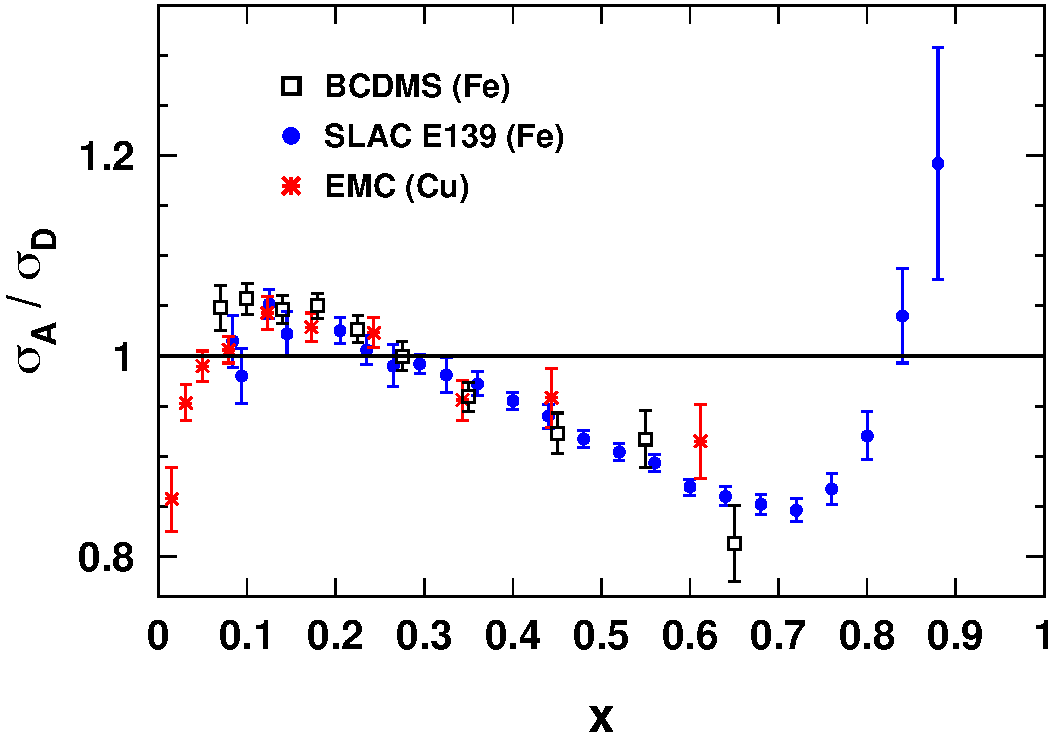
\includegraphics[width=\columnwidth]{emc_cu_fe-crop.pdf}
\caption{EMC effect for iron (BCDMS collaboration~\cite{Benvenuti:1987az} and SLAC E139~\cite{Gomez:1993ri}) and copper (EMC collaboration~\cite{Ashman:1992kv}).
Figure from Ref.~\cite{Guzey:2012yk}.}
\label{fig:emc_iron}
\end{figure}

The EMC effect~\cite{Aubert:1983xm} is the observation that the PDFs for nuclei are different than
the incoherent sum over the PDFs of the constituent nucleons and was the first evidence that 
of the structure of the nucleons may be different when bound together in a nucleus.
Since the original discovery in 1983, there has been a large
program of measurements at several laboratories, such as CERN, Fermilab, SLAC, DESY, and Jefferson Lab (JLab),
aimed at understanding the properties and probing the origin of the nuclear dependence of inelastic
structure functions, covered in detail in several reviews~\cite{Arneodo:1992wf,Geesaman:1995yd,Sargsian:2002wc,Malace:2014uea, Hen:2016kwk}.
Measurements with high energy muon beams (on the scale of 100~GeV) have provided high-precision data at low to
moderate $x$ ($<0.3$), while more modest energy electron facilities (on scale of 10 GeV) have provided
the highest precision at large $x$ ($>0.3$), Fig.~\ref{fig:emc_iron}.  The low-to-moderate $x$
regions show interesting shadowing and anti-shadowing behaviors, while the suppression of the
per-nucleon cross section for $0.3<x<0.7$ is the hallmark of the EMC effect.

\begin{figure}[tbp]
\centering\includegraphics[width=\columnwidth]{plots/e03103_slopes.pdf}
\caption{Size of the EMC effect, in this case assumed to be the slope $|dR/dx|$ between $x=0.35-0.70$, vs. scaled nuclear density. Figure adapted from Ref.~\cite{Seely:2009gt}.}
\label{fig:emc_jlab_hallc}
\end{figure}

The most comprehensive data sets with high precision at large $x$ come from SLAC E139~\cite{Gomez:1993ri} and JLab E03-103~\cite{Seely:2009gt}. The SLAC experiment
measured the EMC effect for a wide range of nuclei, from $^4$He to Au with good precision up to
$x\approx0.8$.  One of the outcomes of E139 was an investigation of the detailed nuclear dependence of the EMC
effect. It was found that the nuclear dependence of the EMC effect at $x \gtrsim =0.6$ is consistent
with both a logarithmic $A$ dependence or a linear dependence on average nuclear density (often parametrized as an $A^{1/3}$ dependence).

The SLAC and early high energy measurements showed a number of global properties of the EMC effect:
%
\begin{itemize}
\item{The shape of the EMC effect (shadowing, anti-shadowing, and EMC regions at small, moderate, and large $x$ respectively) is universal and observed in all nuclei.}
\item{The EMC effect displays little $Q^2$ dependence over the full $x$ range.}
\item{At small $x$ and large $x$, the EMC effect grows with $A$, while there is little apparent $A$ dependence in the anti-shadowing region.}
\end{itemize}
%
Since the first observation of the EMC effect, many theoretical models have been proposed and can be subdivided into two categories.  One includes only ``traditional'' nuclear physics effects, using convolution models with binding effects, detailed models of the nucleon momentum distribution, or pion-exchange contributions. The other category invokes more exotic explanations such as re-scaling of quark distributions in the nuclear environment, contributions of six or nine
quark bags, or modification of the internal structure of the nucleons such as ``nucleon swelling'' or suppression of point-like nucleon configurations. Several reviews give an overview of models of the EMC effect~\cite{Geesaman:1995yd, Norton:2003cb, Piller:1999wx, Hen:2013oha, Malace:2014uea}.


%===============================================================================
\begin{figure}[tbp]
\centering\includegraphics[width=\columnwidth]{plots/plotfit_all_norescaling_nocm_rean_final.pdf}
\caption{Size of the EMC effect plotted vs. the SRC ratio $a_2$. Data are from JLab and SLAC. Figure
from Ref.~\cite{Arrington:2012ax}.}
\label{fig:emc_src_bff}
\end{figure}
%===============================================================================

%===============================================================================
%===============================================================================
\subsection{EMC effect results from Jefferson Lab and the EMC-SRC correspondence}

The primary goal of Jefferson Lab E03-103 was to augment the results obtained from SLAC E139 by taking
advantage of improved target technologies to provide higher precision data for $^4$He, and the first
measurement of the EMC effect from $^3$He at large $x$.  Additional light (Be and C) and heavy (Cu and Au)
targets were also used to provide improved precision at large $x$.

The EMC effect was described using the ratio $R$ of the measured nucleus cross section and deuterium
normalized to the relative number of nucleons.
Since the shape of the EMC effect is universal, the E03-103 analysis assumed the ``size'' of the EMC
effect as the slope of a linear fit of $R$ between $0.35<x<0.7$.  This definition reduces sensitivity to
normalization uncertainties and results in higher sensitivity to the nuclear dependence.

The slope $R$ from E03-103 for $^3$He, $^4$He, Be, and C plotted against scaled nuclear
density is shown in Fig.~\ref{fig:emc_jlab_hallc}.  The nuclear dependence was found to be consistent
with a simple density dependence, with the exception of $^9$Be,  which showed an anomalously larger-than-expected 
EMC effect given its low average nuclear density.  However, if the size of the EMC effect is
governed by the local nuclear density experienced by the quarks in the bound nucleon, rather than the
average density~\cite{Seely:2009gt, PhysRevC.82.054614} a different size of the EMC effect would be predicted.

%===============================================================================
\begin{figure*}[tbp]
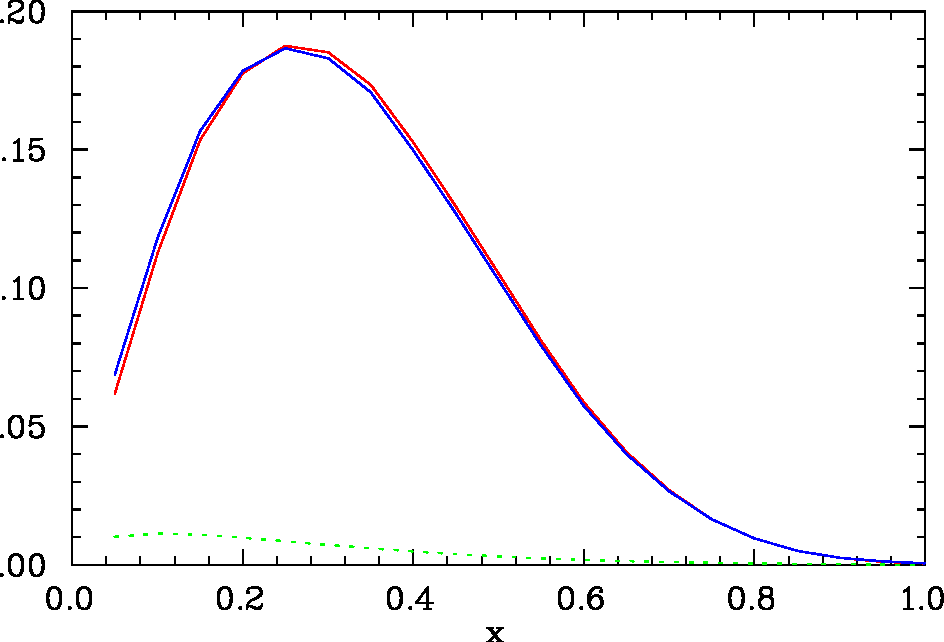
\includegraphics[width=1.0\columnwidth]{plots/qofx2_lin_5per} \hfill
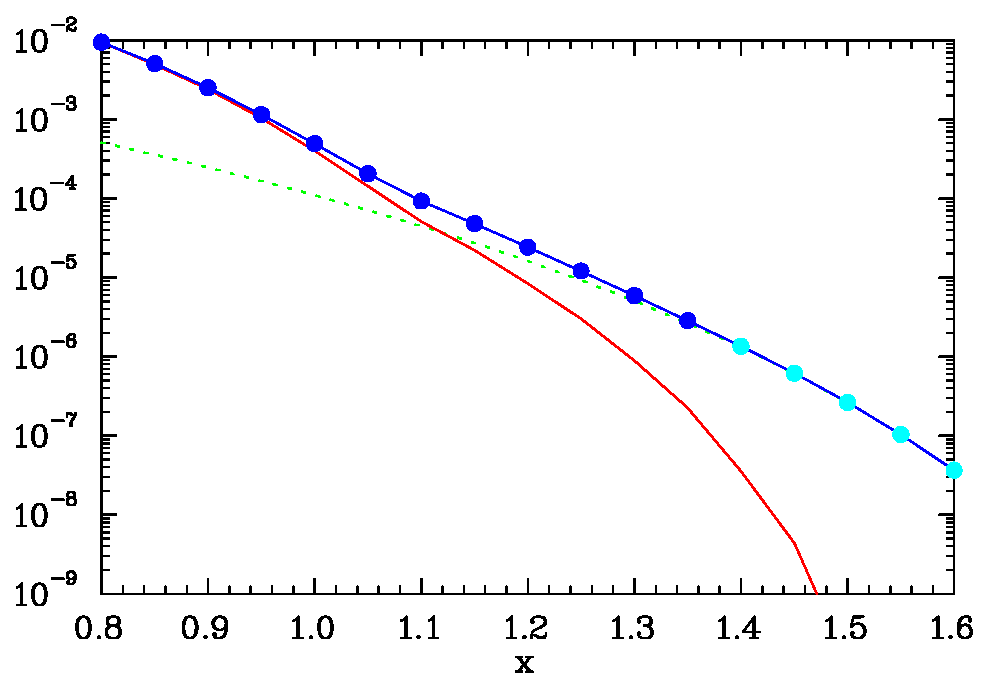
\includegraphics[width=1.0\columnwidth]{plots/qofx2_log_5per}
\caption{This figure is from Ref.~\cite{Arrington:2003qt}, and presents quark distribution calculations for the deuteron, where the dashed line shows 2N components, the dotted line corresponds to a 5\% contribution from 6-quark bags, and the solid blue line shows the sum of the two~\cite{Mulders:1983au}. }
\label{fig:quarkbags}
\end{figure*}
%===============================================================================

When the EMC effect was compared to the unnormalized ratio $a_2=\sigma_A/\sigma_D$~\cite{Frankfurt:1993sp} of the
inclusive cross sections at $x>1$ (which is sensitive to the ``number of short range correlations''
found in a nucleus) a linear correlation between the two quantities was observed~\cite{Weinstein:2010rt}.
This correspondence was even more compelling when $x>1$ ratios for $^9$Be from JLab experiment E02-019 became
available and the same correlation persisted~\cite{Arrington:2012ax, Hen:2012fm}, Fig.~\ref{fig:emc_src_bff}.

The origin of this correspondence is unclear, whether short-ranged correlations (SRCs) in some way cause the EMC effect, or if the two
phenomena are caused by some common underlying source.  A study was conducted to examine whether
both the EMC effect and SRCs are correlated with other independent variables~\cite{Arrington:2012ax}, such
as average nucleon separation energy, with no clear common origin or factor found.  Separate calculations have been 
published using effective field theory which show this is a natural consequence of scale separation~\cite{PhysRevLett.119.262502}.

A subtlety exists in correlation studies between $x>1$ inclusive cross section ratios and the EMC effect. The former represent the relative number of high-momentum nucleons found in a nucleus of mass number $A$ to $A=2$, and not the relative number of nucleon-nucleon pairs.  This means that a causal relationship between high-virtuality nucleons and the EMC effect can potentially represent a different scenario than one where the high-density configurations (SRC pairs) are the culprit.  Additionally, observed $NP$ dominance in SRC experiments~\cite{Subedi:2008zz} implies that for the virtuality hypothesis that the EMC effect may differ for protons and neutrons for non-isoscalar nuclei.

%===============================================================================
%===============================================================================
\subsection{Quarks at $x>1$}
Quasielastic kinematics at $x>1$ probe moving nucleons, but at larger $Q^2$, the inelastic contribution begins to dominate, giving access to quark distributions. Existing JLab data have a limited range in $x$ and require the application of the of so-called "target-mass corrections" (TMCs) to extract the $Q^2 \to \infty$ structure function limit.  This analysis was done for the E02-019 data, showing that the data are approaching the scaling regime~\cite{Fomin:2010ei}.  Here potential 6-quark configurations could result in a noticeable enhancement of the measured cross sections at $x>1$, and be related back to the EMC region where the enhancement is harder to determine.  Fig.~\ref{fig:quarkbags} from Ref.~\cite{Arrington:2003qt} shows the potential effect on the quark distributions in the EMC and the $x>1$ region.

